\documentclass{article}
\usepackage{graphicx} % Required for inserting images
\usepackage{float}
\usepackage[T1]{fontenc}
\usepackage{amsmath}
\usepackage[margin=1in]{geometry}
\usepackage{booktabs}
\usepackage{tabularx}
\usepackage[hidelinks]{hyperref}

\title{Laddering more positions on the SPY gamma book}
\author{Experiment report \textperiodcentered{} L/S Gamma Desk, QUANTT}
\date{2026-10-16}

\begin{document}

\maketitle

\textbf{Question:} With the live rules, does net P\&L peak at an interior number of open same-side positions (between 1 and 8, laddered one per signal run), at both 1x and 2x spreads?

\textbf{Method:}

\begin{itemize}

\item Pre-registered backtest. The hypothesis card was committed before any run (commit e5e0806).

\item The live paper rules (\texttt{configs/\allowbreak{}paper.\allowbreak{}toml}) are replayed on R2 replay snapshots v1 (config\_hash b040760187f0) over the development window 2014-06-02 to 2024-12-31. The hold-out (2025-01-01 to 2026-07-10) was not used.

\item New research-only switch \texttt{[backtest] max\_\allowbreak{}positions}, committed in 25b6fc2 (live holds one position and does not read it):

\begin{itemize}

\item While the signal stays on one side, the engine opens one more position per 10:15 run, up to N.

\item Each position has its own expiry, strike, premium, and time, stop and profit exits. A flip or flat signal closes all of them.

\item Hedges are netted into one share order per run.

\item With N = 1 the engine reproduces baseline trial 1 exactly.

\end{itemize}

\item Variants: \texttt{max\_\allowbreak{}positions} = 2, 3, 4, 6, 8. N = 1 is baseline trial 1.

\begin{itemize}

\item N = 8 is the Reg-T limit for \$250k: one short put plus its hedge needs at most about \$31k.

\end{itemize}

\item Every variant ran once at 1x and 2x spreads. Costs: \$0.65 per contract and \$0.005 per share, with a \$1 minimum per order.

\end{itemize}

This report was written by Claude at the PM's request.

\section{Result vs the pass bar}

Every check had to hold at 1x and 2x. P\&L is net USD on daily equity, 1 contract per position.

\begin{center}\small
\begin{tabularx}{\linewidth}{>{\raggedright\arraybackslash}X l l >{\raggedright\arraybackslash}X l}
\toprule
\textbf{Check} & \textbf{1x value} & \textbf{2x value} & \textbf{Bar} & \textbf{Result} \\
\midrule
N with the highest full-window P\&L & 1 & 1 & interior (2, 3, 4 or 6) & fail \\
Peak minus the better end (N = 1 or 8) & \$0 & \$0 & \ensuremath{\geq} \$500 & fail \\
N with the highest P\&L, 2014-2019 & 1 & 1 & interior & fail \\
N with the highest P\&L, 2020-2024 & 1 & 1 & interior & fail \\
Event floor: ladder entries at N = 8 (1x) & 328 &  & \ensuremath{\geq} 30 & met \\
\bottomrule
\end{tabularx}
\end{center}

\textbf{Verdict: failed.} Net P\&L is highest at N = 1 at both spreads and in both halves. Laddering happened often (328 ladder entries at N = 8), so this is a real result, not a lack of events. The curve is not a hump. At 1x it falls from N = 1 to N = 3, stays flat to N = 6 and recovers a little at N = 8. At 2x it keeps falling to N = 6.

\subsection{Full-window numbers (not part of the bar)}

\begin{center}\small
\begin{tabularx}{\linewidth}{>{\raggedright\arraybackslash}X l l l l l l}
\toprule
\textbf{max\_positions} & \textbf{1} & \textbf{2} & \textbf{3} & \textbf{4} & \textbf{6} & \textbf{8} \\
\midrule
Net P\&L 1x & \ensuremath{-}2,060 & \ensuremath{-}4,586 & \ensuremath{-}6,433 & \ensuremath{-}6,118 & \ensuremath{-}6,836 & \ensuremath{-}5,807 \\
Net P\&L 2x & \ensuremath{-}4,122 & \ensuremath{-}7,970 & \ensuremath{-}10,699 & \ensuremath{-}10,944 & \ensuremath{-}12,450 & \ensuremath{-}11,974 \\
Sharpe on \$250k, 1x & \ensuremath{-}0.36 & \ensuremath{-}0.44 & \ensuremath{-}0.44 & \ensuremath{-}0.35 & \ensuremath{-}0.30 & \ensuremath{-}0.21 \\
ES 5\% (daily), 1x & \ensuremath{-}96.5 & \ensuremath{-}177.2 & \ensuremath{-}243.4 & \ensuremath{-}291.5 & \ensuremath{-}370.9 & \ensuremath{-}426.3 \\
Max drawdown 1x & 3,027 & 5,011 & 6,809 & 6,792 & 7,773 & 7,404 \\
Round trips & 131 & 220 & 282 & 331 & 400 & 449 \\
Hedge orders & 914 & 939 & 940 & 941 & 942 & 941 \\
Peak est. Reg-T margin (\$k) & 31 & 61 & 90 & 116 & 162 & 192 \\
\bottomrule
\end{tabularx}
\end{center}

\section{Charts}

\begin{figure}[H]\centering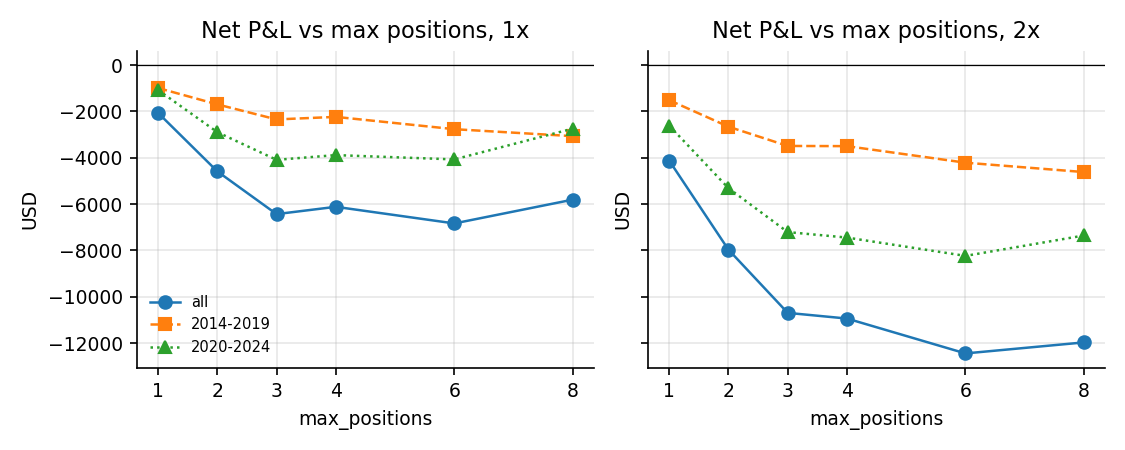
\includegraphics[width=0.92\linewidth]{figures/pnl_vs_n.png}\caption{Net P\&L against max\_positions, full window and both halves, at 1x and 2x}\end{figure}

The pass-bar chart. At 1x every line starts highest at N = 1. The full-window and 2020-2024 lines bend back up at N = 8 (2020-2024: \ensuremath{-}\$2,741 against \ensuremath{-}\$1,073 at N = 1, still lower), and the 2014-2019 line bends slightly at N = 4. At 2x every line falls almost all the way.

\begin{figure}[H]\centering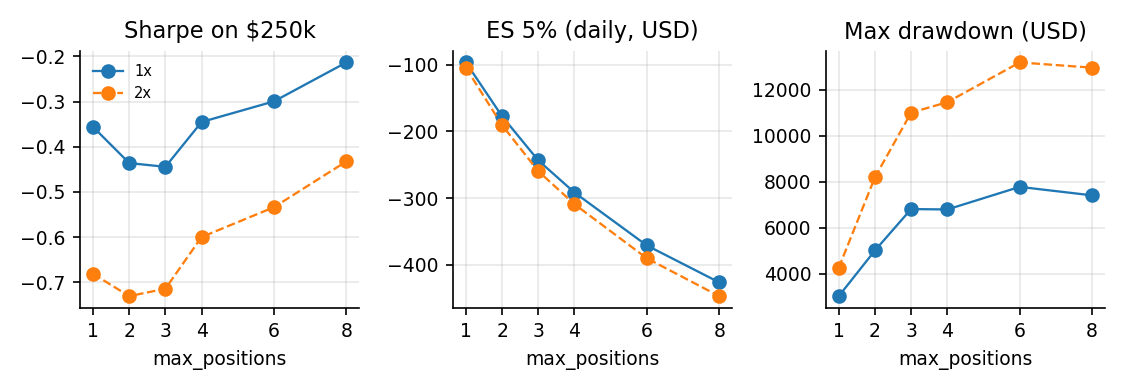
\includegraphics[width=0.92\linewidth]{figures/risk_vs_n.png}\caption{Sharpe on \$250k, daily ES 5\% and maximum drawdown against max\_positions}\end{figure}

Tail risk grows steadily with N, a little less with each extra position: ES goes from \ensuremath{-}\$97 to \ensuremath{-}\$426 a day at 1x. Sharpe is not monotone (\ensuremath{-}0.36, \ensuremath{-}0.44, \ensuremath{-}0.44, \ensuremath{-}0.35, \ensuremath{-}0.30, \ensuremath{-}0.21 at 1x). It gets less negative at large N because the volatility of daily P\&L grows about 4.7x while the average daily loss grows about 2.8x. That is not a better book: the loss grows, and the noise grows faster.

\begin{figure}[H]\centering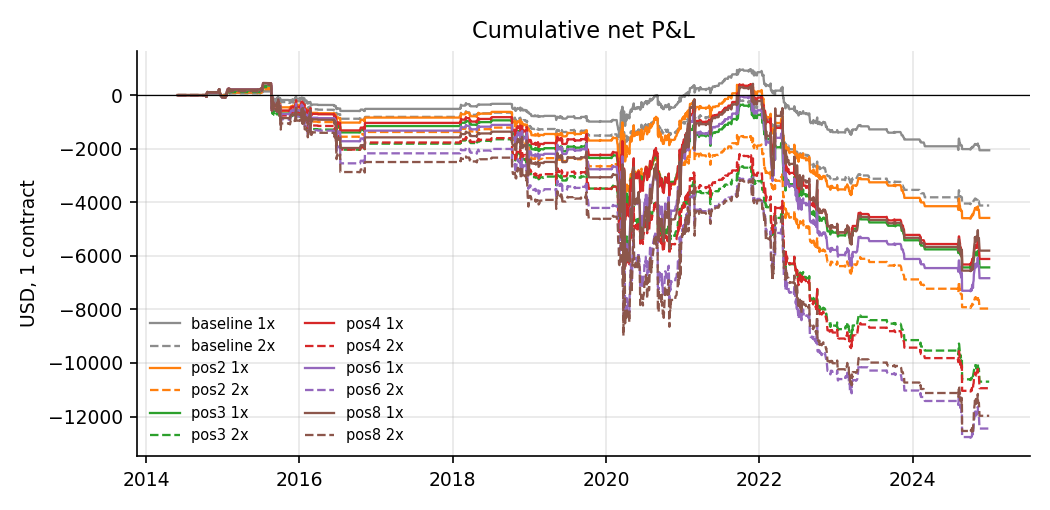
\includegraphics[width=0.92\linewidth]{figures/cum_pnl.png}\caption{Cumulative net P\&L, 1x solid and 2x dashed; baseline grey}\end{figure}

All variants follow the same path, scaled by exposure. The gap opens in 2015-2016, in 2018, and above all in 2022, when the 1x loss grows from \ensuremath{-}\$2,242 (N = 1) to \ensuremath{-}\$5,215 (N = 6).

\begin{figure}[H]\centering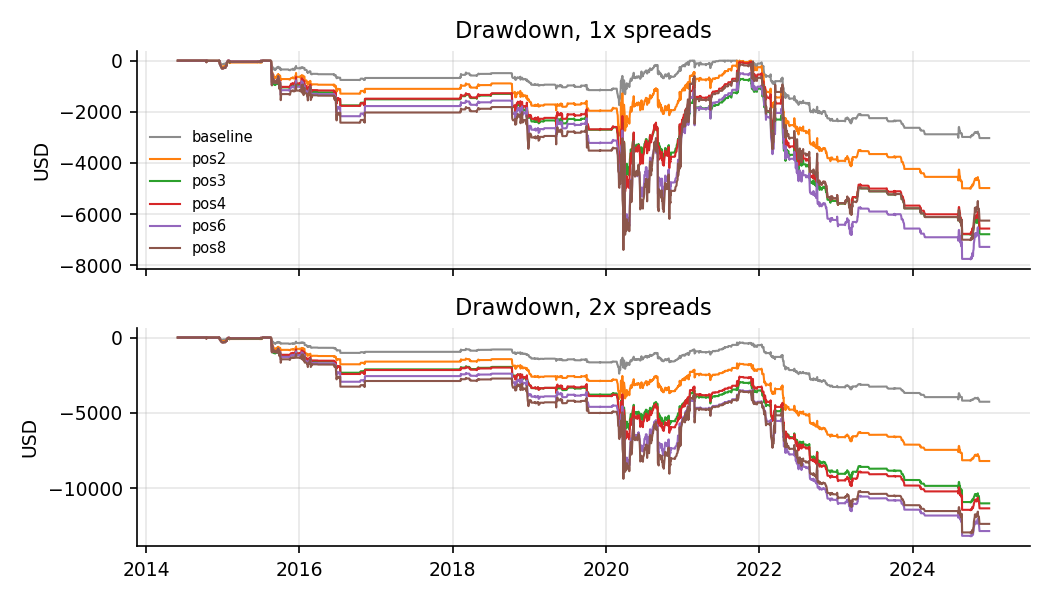
\includegraphics[width=0.92\linewidth]{figures/drawdown.png}\caption{Drawdown at 1x and 2x spreads}\end{figure}

For most N the trough of the deepest drawdown is in October-November 2024. For N = 1 and 2 at 1x it comes after the 2021 peak. For the others, and for every N at 2x, the high-water mark is still mid-2015. The exception is N = 8 at 1x, whose trough is the March 2020 crash (2020-03-24). At 2x, N = 6 and 8 run past \$12,000.

\begin{figure}[H]\centering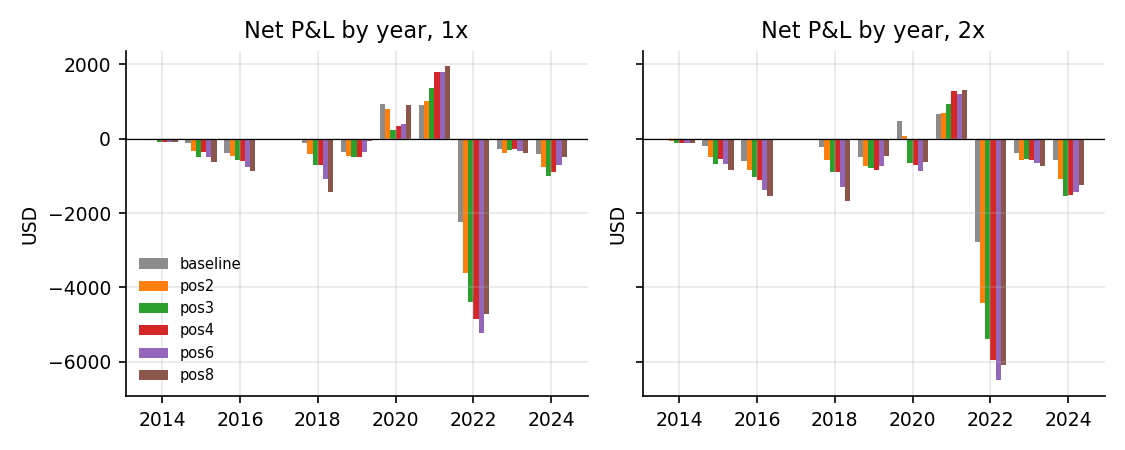
\includegraphics[width=0.92\linewidth]{figures/yearly.png}\caption{Net P\&L by year}\end{figure}

Laddering helps clearly in 2021 (+\$904 at N = 1 to +\$1,947 at N = 8), and at N = 8 in 2019 (\ensuremath{-}\$65 against \ensuremath{-}\$349). 2020 is about even at N = 8 (+\$899 against +\$939) and lower in between. Every other losing year gets worse, most of all 2022.

\begin{figure}[H]\centering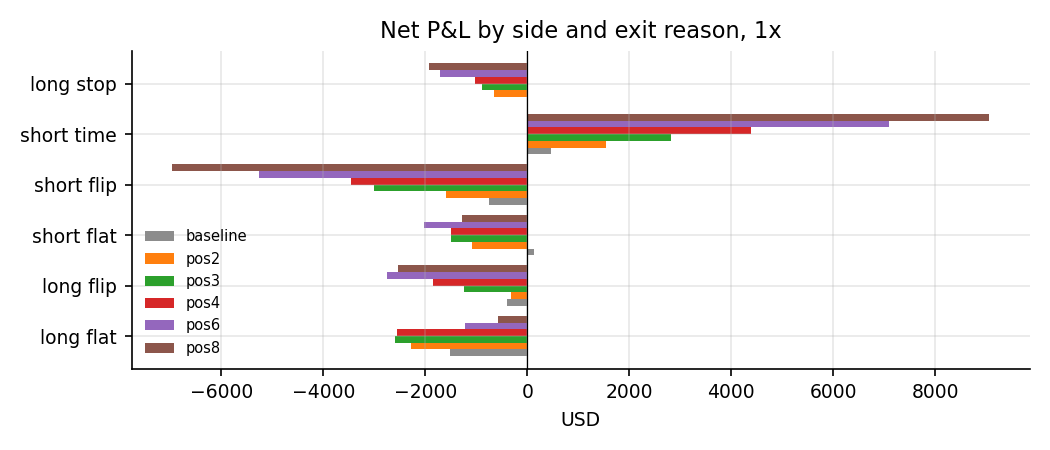
\includegraphics[width=0.92\linewidth]{figures/by_reason.png}\caption{Net P\&L by side and exit reason, 1x}\end{figure}

The cost of laddering shows up in two places. Shorts closed by a flip signal lose \ensuremath{-}\$6,959 at N = 8 against \ensuremath{-}\$745 at N = 1. Long trades lose far more than at N = 1 at every N (\ensuremath{-}\$5,035 at N = 8 against \ensuremath{-}\$1,913). Short time exits are the gain: +\$9,052 at N = 8 against +\$470. These are round-trip totals (see the note under Analysis).

\begin{figure}[H]\centering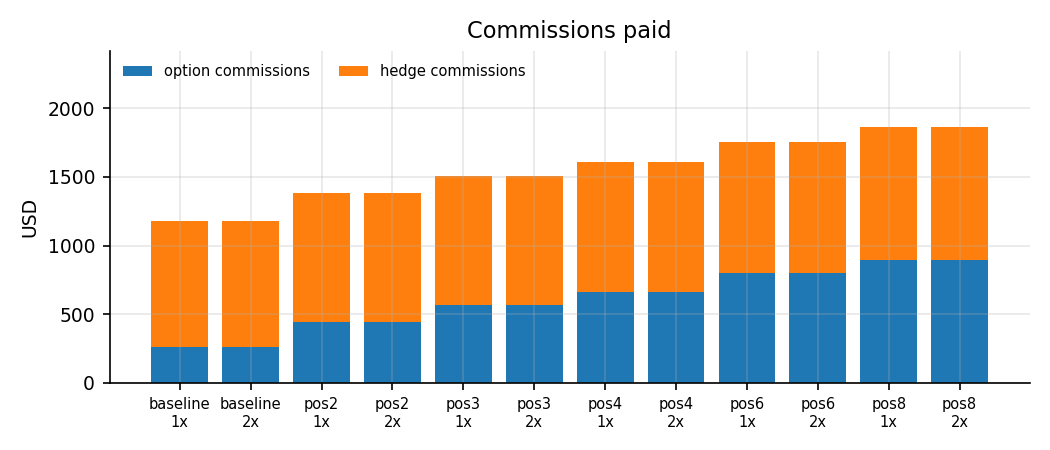
\includegraphics[width=0.92\linewidth]{figures/fees.png}\caption{Commissions paid}\end{figure}

Hedge orders barely change (914 to 941), because netting keeps one share order per run. Option commissions grow with the number of round trips (\$262 to \$898).

\begin{figure}[H]\centering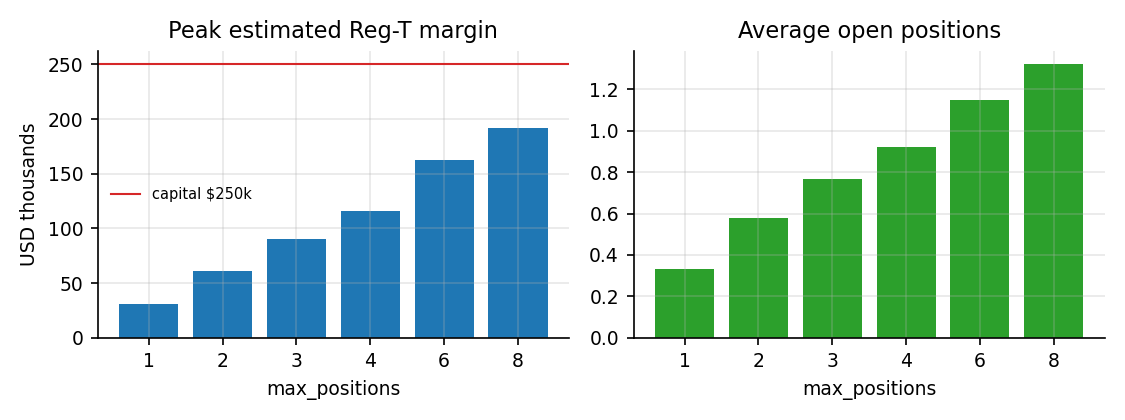
\includegraphics[width=0.92\linewidth]{figures/margin.png}\caption{Peak estimated Reg-T margin and average open positions against max\_positions}\end{figure}

Every N fits in \$250k: the peak estimated Reg-T margin is \$192k at N = 8. On average the book holds only 0.3 to 1.3 positions, because the signal is flat most of the time.

\section{Analysis}

Laddering scales the book's exposure to what the signal is doing at the time. It doesn't change the signal's edge, which is negative overall. So the curve mostly shows the baseline loss scaled up. Two effects make it bend instead of falling in a straight line.

\begin{itemize}

\item \textbf{Longs lose at every rank.} Long positions lose about \$57-63 each at N = 8, whether they are the first, second, or third and later position (\ensuremath{-}\$5,035 in total at 1x). Laddering into long signals only adds more of a losing trade. This repeats the finding of \texttt{2026-\allowbreak{}10-\allowbreak{}16-\allowbreak{}short-\allowbreak{}only}.

\item \textbf{Late shorts in a long short-signal run make money.} At N = 8 at 1x, shorts opened as the third or later position made +\$3,207 over 215 trades, mostly through time exits (+\$7,884 of the +\$9,052 short time-exit total). The second-rank shorts lost (\ensuremath{-}\$1,781). The ladder's reach also cuts the other way: when the signal flips to long, every short closes at once, and short flips lose \ensuremath{-}\$6,959. The short side nets +\$813 at N = 8 at 1x, but \ensuremath{-}\$3,513 at 2x: the doubled spread cost of its 364 round trips wipes it out.

\end{itemize}

\textbf{A note on attribution:} the side, rank and exit-reason totals are round-trip P\&L. Round-trip P\&L leaves out the order that flattens the hedge after the last position closes, which fills on the fill view (spread and slippage) and carries its own fee. With more positions that order gets bigger. At N = 8 (1x), round trips sum to \ensuremath{-}\$4,222 against \ensuremath{-}\$5,807 of equity P\&L, so \ensuremath{-}\$1,585 is unattributed. About \$2.1k of it follows long closes, so longs are worse than shown and shorts about \$0.5k better. The pass bar uses equity P\&L, which includes everything, and the conclusions don't change.

The bend at N = 8 comes from those late shorts. Their gains sit in 2020 (+\$1,643), 2021 (+\$2,520) and 2024 (+\$857), and they lose in 2015-2016 and 2022. N = 8 does better than N = 6 in 2019 (\ensuremath{-}\$65 against \ensuremath{-}\$359), 2020 (+\$899 against +\$408) and 2024. That rests on the few long short-signal runs that let the ladder fill, so it may not repeat. Nothing in it is close to beating N = 1.

\section{Verdict}

\textbf{Failed} on the pre-registered bar, at both spreads and in both halves. Net P\&L is highest at N = 1. With the current rules, laddering more positions only adds risk (ES up 4.4x at N = 8) without adding P\&L. Keep one position. A hold-out run is not needed.

A possible follow-up, which needs its own card: laddering only short signals. Here late short entries made money at 1x but not at 2x. This idea comes from this run, so it would be in-sample and would need the hold-out.

\section{Caveats}

\begin{itemize}

\item \textbf{In-sample:} the window has been used by five earlier experiments, although the hypothesis itself is the PM's prior.

\item \textbf{One contract per position:} the \$1 minimum still matters for small hedge orders, but netting keeps hedge orders almost flat across N.

\item \textbf{Spread model:} fitted on about two weeks of calm 2026 live quotes. The 2x run is the stress test, and it fails clearly.

\item \textbf{Data gaps:} R2 has no month-end weekdays, so about 3.3\% of scheduled times are skipped (89 at every N).

\item \textbf{Margin estimate:} a simple Reg-T formula, not IBKR's real calculation. Portfolio margin would allow more positions, but every N tested already loses more than N = 1.

\item \textbf{Engine modelling choices} (agreed with the PM before the run):

\begin{itemize}

\item One entry per 10:15 run.

\item Flip and flat close every position.

\item Netted hedge fills are split across positions for stop checks.

\end{itemize}

Other choices could change the shape, for example staggered exits or a minimum gap between entries.

\end{itemize}

\section{Trials}

10 trials for this experiment (5 variants at 1x and 2x, one run of \texttt{experiment.\allowbreak{}py}), plus the baseline's 2. Before the run, the engine change was checked against baseline trial 1 by calling the engine directly. That check is not registered. The pass bar was not changed.

\end{document}
